%!TEX program = xelatex
\documentclass[12pt,letterpaper]{article}
\usepackage[portuguese]{babel}
\usepackage[utf8]{inputenc}
\usepackage[math]{iwona}
\usepackage{setspace}
\usepackage{hyperref}
\usepackage{cite}
\usepackage{url}    
\usepackage{tabularx}
\usepackage{graphicx}
\usepackage[left=4cm,right=2cm,top=3cm,bottom=3cm]{geometry}

%======================================================================

\begin{document}
\onehalfspacing 
\thispagestyle{empty}

\begin{center}
\vspace{0.2cm}

\hrulefill

\textbf{UNIVERSIDADE FEDERAL DE ALAGOAS}\\
\textbf{PRÓ-REITORIA DE PESQUISA E PÓS-GRADUAÇÃO}\\
COORDENAÇÃO DE PESQUISA

\hrulefill

\vspace{0.5cm}

PROGRAMA INSTITUCIONAL DE BOLSAS DE INICIAÇÃO\\ CIENTÍFICA -- PIBIC CNPq/UFAL/FAPEAL

\vspace{1.0cm}

\textbf{\textit{\Large{RELATÓRIO FINAL \\ (2017 -- 2018)}}}\\

\vspace{1.2cm}

\textbf{TÍTULO DO PROJETO DE PESQUISA:}

\underline{Análise de Sinais e Imagens com Distâncias Estocásticas e Diferenças de Entropias}

\vspace{0.6cm}

\textbf{TÍTULO DO PLANO DE TRABALHO:}

\underline{Ferramentas para análise de séries temporais}

\end{center}

\textbf{\underline{NOME DO ORIENTADOR:}} Alejandro César Frery 

\vspace{0.4cm}

\textbf{\underline{NOME DO BOLSISTA:}} Eduarda Tatiane Caetano Chagas

\vspace{1cm}

\begin{table}[!h]
\begin{center}
\begin{tabularx}{\textwidth}{|X|X|X|X|}
\hline                              
\hspace{1.3cm} X & Bolsista CNPq &  &Bolsista FAPEAL\\
\hline             
& Bolsista UFAL &  &Colaborador\\
\hline     
\end{tabularx}
\end{center}
\end{table}

GRANDE ÁREA DO CONHECIMENTO (CNPq): Ciências  Exatas  e  da  Terra

SUB-ÁREA DO CONHECIMENTO (CNPq) : Matemática  da  Computação   

\vspace{0.5cm}

Projeto financiado:  \hspace*{1.5cm} Sim X \hspace*{1.5cm} Não

Órgão financiador dos recursos: \underline{CNPq}

\vspace*{0.8cm}

\begin{center}

Maceió - AL, 15/08/2018

\end{center}

%=================================================================

\newpage
\section*{\centering \textbf{RESUMO}} % (Máximo 1 página – Sem parágrafos) 
%Tem no parcial

	Neste relatório relatamos o desenvolvimento de uma plataforma de análise de séries temporais por meio de descritores causais oriundos da Teoria da Informação, tendo como objetivo facilitar tal estudo nos mais diversos ramos da ciência, como por exemplo, a discriminação entre fenómenos estocásticos e caóticos~\cite{DistinguishingNoiseFromChaos}, a identificação de padrões de comportamento em redes veiculares~\cite{CharacterizationVehicleBehaviorInformationTheory}, a classificação e verificação de assinaturas \textit{online}~\cite{ClassificationVerificationOnlineHandwrittenSignatures}, na análise da robustez de redes~\cite{InformationTheoryPerspectiveNetworkRobustness}, e a classificação de padrões de consumo de energia elétrica~\cite{CharacterizationElectricLoadInformationTheoryQuantifiers}.
    A implementação foi realizada por meio da linguagem de programação \texttt R que além de fornecer ferramentas gráficas, também possui uma grande precisão numérica, ambas as características de extrema importância ao longo deste trabalho.
 Após comentar brevemente a respeito dos objetivos do projeto e a sua importância na análise não-paramétrica de séries temporais, expomos as etapas e os resultados alcançados.\\

\textbf{Palavras-chave:} Séries Temporais, Teoria da Informação, plataforma \texttt R.

%=========================================================

\newpage
\section*{\centering \textbf{INTRODUÇÃO E OBJETIVOS}} %(Máximo 1 página)
%Tem os objetivos

Séries temporais podem ser definidas como qualquer conjunto de dados obtidos a partir de um processo observacional ao longo de um determinado período de tempo, não necessariamente dividido em espaços igualitários, sendo caracterizadas pela dependência serial existente entre seus elementos. 

O estudo de séries temporais é tipicamente dividido em duas vertentes \cite{BrockwellDavis91}, a análise do domínio do tempo e do domínio da frequência, sendo utilizado em ambas abordagens os dados que resultam diretamente das observações coletadas, que por sua vez estão sujeitos a efeitos danosos de diversos tipos de contaminação. 
Uma solução alternativa, presente na literatura, para evitar os efeitos dessa contaminação, consiste no uso de métodos não-paramétricos.

O projeto objetiva facilitar a análise não-paramétrica de séries temporais, desenvolvendo um sistema de extração dos descritores causais oriundos da Teoria da Informação que auxiliam no processo de identificação do tipo de dinâmica subjacente aos dados. Desse modo, são objetivos específicos deste trabalho de pesquisa:

\begin{itemize}
\item Implementar funções de análise de séries temporais utilizando descritores da Teoria da Informação;
\item Implementar uma interface gráfica amigável para a aplicação de tais funções;
\item Manter a portabilidade do software para os diversos sistemas operacionais e arquiteturas de hardware;
\item Desenvolver tal projeto a partir do uso de ferramentas FLOSS (\textit{Free/Libre Open Source Software});
\item Validar a interface e as funções com usuários finais.
\end{itemize}

%=========================================================

\newpage
\section*{\centering \textbf{METODOLOGIA}} %(Máximo 2  páginas)
%Etapas do plano de trabalho

A metodologia foi dividida em duas etapas, a etapa teórica e a implementação das funcionalidades.
Esta consiste em um processo de pesquisa específico, onde foi realizada a partir da análise de artigos e textos científicos, visando ampliar os conhecimentos sobre o tema proposto. 

Foram estudados ao longo deste momento, temas como séries temporais e as suas propriedades, Teoria da Informação, entropias~\cite{salicruetal1993}, distâncias estocásticas~\cite{StatisticalInferenceBasedonDivergenceMeasures} e a linguagem de programação \texttt R.

O estudo das funções a serem implementadas foi realizado a partir da análise de um conjunto de referências bibliográficas de qualidade, visando ampliar os conhecimentos a cerca do tema proposto. 
Após o término da revisão bibliográfica da literatura existente, foi então dado início a implementação do sistema em \textit{R}, onde por meio do software livre de desenvolvimento integrado RStudio Desktop, foi possível acompanhar os crescentes avanços no âmbito gráfico e desenvolver todo o código do referente projeto.

Para que tal ferramenta seja aplicada na análise de dados é de suma importância realizar a verificação de suas propriedades numéricas. 
Portanto, a avaliação da qualidade numérica das funcionalidades desenvolvidas foi feita utilizando uma metodologia própria baseada em sistemas dinâmicos com saídas conhecidas.

Foi então realizada uma pesquisa sobre as alternativas existentes para o desenvolvimento da interface gráfica do projeto, considerando os seguintes fatores: portabilidade do software para os diversos sistemas operacionais e arquiteturas de hardware, e integração com a linguagem de programação \texttt R.

\texttt{RGtk2} e \texttt{Java Swing} foram as alternativas iniciais para o desenvolvimento da interface gráfica. 
No entanto, após estudos sobre o funcionamento destas GUIs (\textit{Graphical User Interface}), optamos pelo \texttt{RGtk2}, por ser uma biblioteca própria do ambiente de desenvolvimento \texttt R e pela maior facilidade em manter a portabilidade do sistema.

Foram desenvolvidos alguns protótipos de modelos de interface com as alternativas de bibliotecas gráficas citadas anteriormente, sempre com foco na experiência do usuário.

Após a escolha da biblioteca \texttt{RGtk2}, fizemos a integração entre o ambiente gráfico e as funções de análise de séries temporais implementadas anteriormente.

Ao longo do desenvolvimento do projeto foram escritos manuais e tutoriais de uso.

%=========================================================

\newpage
\section*{\centering \textbf{RESULTADOS E DISCUSSÕES}} %(máximo 4 páginas)
%Apresentação e discussão dos resultados

Há diversas ferramentas que auxiliam na análise clássica de séries temporais; para a plataforma \texttt R, existindo diversas bibliotecas para essa finalidade (ver \url{https://cran.r-project.org/web/views/TimeSeries.html}). 
Além destas opções, o usuário também pode contar com os softwares de visualização de séries temporais. 
No entanto, são limitadas as opções de bibliotecas e softwares que trabalham exclusivamente com técnicas não-paramétricas.

Apresentamos assim o desenvolvimento de uma ferramenta portável, rápida e de boa qualidade numérica que possibilita gerar novos métodos de interação do usuário com o sistema de análise, permitindo que este seja capaz de analisar os diferentes descritores oriundos da Teoria da Informação e permitir a análise gráfica dos resultados.

Seguindo o modelo de engenharia de software em espiral, o sistema foi projetado e desenvolvido de forma modular, composto pelas seguintes unidades:

\begin{itemize}
\item Módulo de simbolização;
\item Módulo de análise;
\item Modulo de visualização e interação (Em fase de desenvolvimento););
\end{itemize} 

Esses módulos foram então desenvolvidos seguindo um cronograma. 
Depois passaram pelas seguintes etapas:

\begin{itemize}
\item Integração dos módulos em um sistema;
\item Teste e validação do sistema (em fase de desenvolvimento);
\item Geração da interface gráfica (em fase de desenvolvimento).
\end{itemize}

Permite-se a leitura de dados em vários formatos (TXT, CSV ou XLSX), e o usuário a seguir poderá escolher:

\begin{itemize}

	\item Gerar o gráfico da série (ver Figura 1);
	\item Calcular seus diversos valores de Entropia;
	\item Calcular seus diversos valores de Distâncias Estocásticas;
	\item Calcular complexidades estatísticas;
    \item Identificar padrões no gráfico da série temporal;
    \item Gerar planos de Entropias;
    \item Gerar planos de Distâncias Estocásticas;
	\item Gerar o histograma de padrões (ver Figura 1);
	\item Identificar o ponto característico da série no plano Entropia-Complexidade (ver Figura 1).

\end{itemize}

Um elemento original do sistema é a vinculação entre o histograma de padrões, formados através do processo de \textit{simbolização de Bandt \& Pompe}~\cite{PermutationEntropyBandtPompe}, e a série temporal. 
Escolhendo um ou mais elementos do histograma, os valores correspondentes na série temporal aparecem realçados. 
Esta funcionalidade permite a análise visual da distribuição temporal dos padrões, possibilitando futuramente a realização de outros testes.
 
O teste e a validação do sistema são tarefas contínuas, bem como o desenvolvimento de novas funcionalidades. 
  
\begin{figure}[!ht]
	\centering
	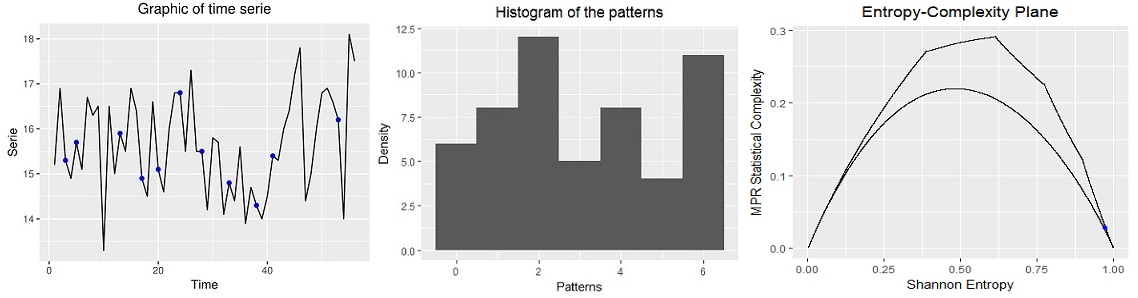
\includegraphics[width=1\columnwidth]{rplot}        
    \caption{Representação gráfica da análise de uma série temporal de produção anual de cevada por acre.}
\end{figure}
 
\begin{figure}[!ht]
	\centering
	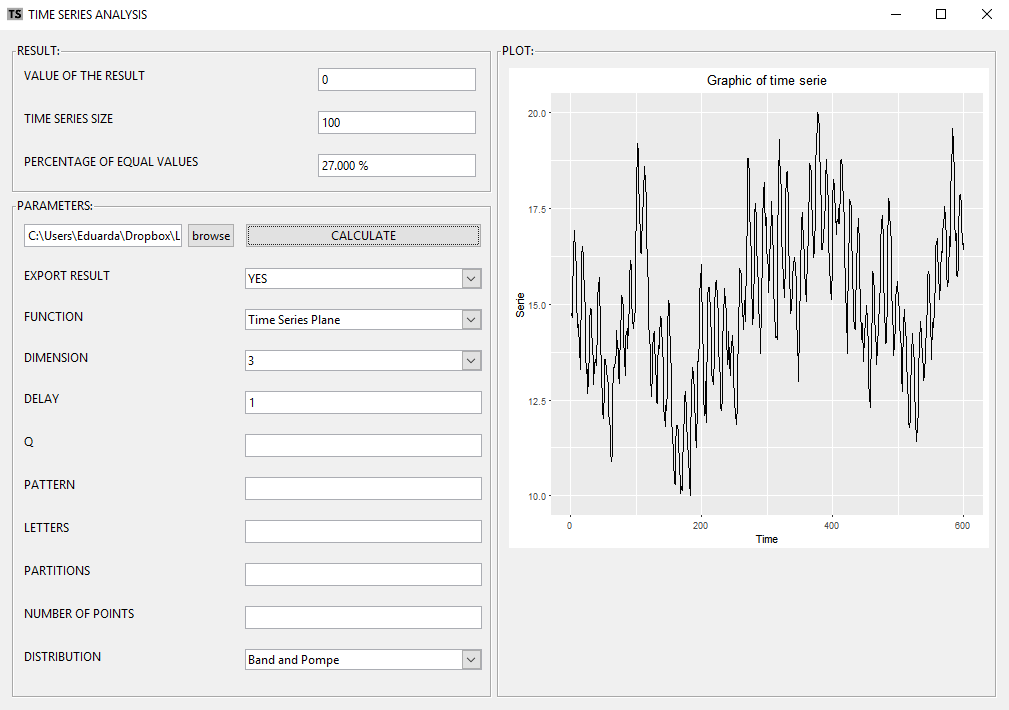
\includegraphics[width=0.95\columnwidth]{TMS}   
    \caption{Imagem atual do software desenvolvido ao longo do projeto.}
    \vspace{6cm}
\end{figure}

\vspace*{9cm}

%=========================================================

\section*{\centering \textbf{CONCLUSÕES}} %(máximo 2  páginas)

 Através do desenvolvimento de tal plataforma por meio da linguagem \textit{R}, fornecemos a base de geração de inúmeros outros modelos que tenham como objetivo a implementação de sistemas confiáveis que tornem mensuráveis as variadas propriedades presentes na teoria da informação, facilitando não apenas o estudo de séries temporais, como também todo o ramo atuante de análise de dados estatísticos.

Utilizando a linguagem \textit{R} e seus benefícios poderemos trabalhar com processamento de imagens de modo prático e eficiente, sendo a motivação para futuros trabalhos abranger tal proposta à análise não apenas de arquivos de dados, mas também proporcionando a extração de séries presentes em texturas.

%=========================================================

\newpage
%REFERÊNCIAS BIBLIOGRÁFICAS (máximo 2  páginas)

\bibliographystyle{unsrt}
\bibliography{./ref}

%=========================================================

\newpage

\section*{\centering \textbf{PLANO DE TRABALHO INDIVIDUAL E DIFERENCIADO}} %(igual projeto original) 2 páginas

\textbf{Objetivos do trabalho da estudante:} Implementar funções de análise de séries temporais utilizando descritores da Teoria da Informação; implementar uma interface para a aplicação dessas funções; validar a interface e as funções com usuários finais.

\textbf{Metodologia correspondente:} Usaremos a plataforma \textit{R}. Verificaremos a qualidade numérica das funções implementadas utilizando um protocolo próprio baseado em sistemas dinâmicos que possuem saídas conhecidas. A estudante analisará alternativas para a implementação da interface. Adotaremos uma versão do Modelo em Espiral de desenvolvimento de software, adaptado às necessidades do software científico.

\textbf{Cronograma de atividades:}

\textbf{Atividade 1:} Estudo das funções a serem implementadas

\textbf{Atividade 2:} Implementação e validação numérica

\textbf{Atividade 3:} Análise de alternativas para o desenvolvimento da interface

\textbf{Atividade 4:} Desenvolvimento de protótipos

\textbf{Atividade 5:} Versão de produção da interface

\textbf{Atividade 6:} Validação, verificação e preparação de manuais e tutoriais de uso


\begin{figure}[!ht]
	\begin{center}
		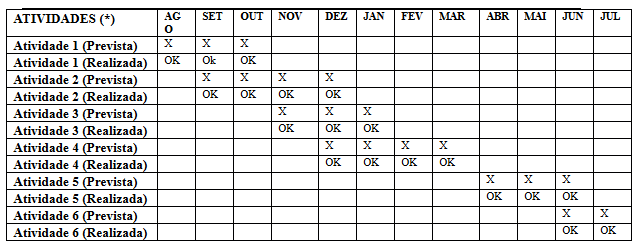
\includegraphics[width=0.95\columnwidth]{tabela}
	\end{center}
\end{figure}

\end{document}
